\frontmatter
\title{Matroid Theory}
\author{Héctor Manuel Téllez Gómez}
\date{January 27, 2014 - \today}
\maketitle

\tableofcontents

\mainmatter
\chapter*{Note for the readers:}
    The goal on writing this in english instead of writing it in my first language (spanish) is because 
    this way I can start building a portfolio that could not be as important as a research project, but
    it is work after all. So it would be better to have something to show that nothing to show at all, 
    and much better if the audience capable of read it is as wide as possible.\pn
    
    As my first language is not english, this text could have a lot of mispellings and
    bad use of english. I apologize in advance and I'll try to be as careful as possible.\pn
    
    Here is a link to this project's version controller repository:\par
    \href{https://github.com/tellezhector/matroids}{https://github.com/tellezhector/matroids}\par
    There you can see what are the changes that have ocurred along all this project's lifetime.\pn
    
    If you want to leave comments you can do it there, where anyone else is able to notice it. Or you could 
    write directly to my personal e-mail address, which is: \texttt{tellez.hector@gmail.com} where it will be read only
    by me.

\chapter{Union Of Closed Sets That Is Not Closed}
\begin{definition}[Closure]
    Given a matroid $M=(E,\c{J})$ with rank function $f$. The \textbf{closure} of a set $S \subset E$
    is
    \begin{align}
        Cl(S) = \{ x \in E | r(S \cup \{ x \} ) = r(S)\}.
    \end{align}    
\end{definition}

\begin{definition}[Closed set]
    Given a matroid $M=(E,\c{J})$ with rank function $f$. We say that a set $S \subset E$ is \textbf{closed}
    if
    \begin{align}
        Cl(S) = S.
    \end{align}
\end{definition}

\prob
{
    Give an example of two closed sets whose union is not closed.
}

\begin{proof}
    We are going to use the linear matroid of $\Z^2$, where the independent sets are 
    $$\emptyset, \{(1, 0)\}, \{(0, 1)\}, \{(1, 1)\}, \{(1, 0), (0, 1)\}$$
    and the rank function is the size of the biggest independent set contained.\pn
    
    It is clear that $A = \{(1, 0), (0, 0)\}$ and $B = \{(0, 1), (0, 0)\}$ are both closed.
    But $C = A \cup B = \{(1, 0), (0, 1), (0, 0)\}$ is not, because $r(C) = 2 = r(C \cup \{ (1, 1) \})$ and
    $(1, 1) \not\in C$.
\end{proof}

\chapter{First Test}
    \begin{center} February 17, 2014 \end{center}
    Test for Oxley's book first chapter (Basic definitions and examples). 
    
    \section{Oxley, Section 1.1, Problem 2}
        \prob{
    Let A be the matrix
    $$\bordermatrix{
            &   1   &   2   &   3   &   4   &   5   &   6   \cr
            &   1   &   0   &   0   &   1   &   1   &   0   \cr
            &   0   &   1   &   0   &   1   &   0   &   1   \cr
            &   0   &   0   &   1   &   0   &   1   &   1   
    }$$

    For q in $\{2,3\}$, let $M_q[A]$ be the vector matroid of $A$ when $A$ is viewed over $GF(q)$,
    the field of $q$ elements. Show that:

    \begin{enumerate}
        \item[(i)] 
            The sets of circuits of $M_2[A]$ and $M_3[A]$ are different.
        \item[(ii)]
            $M_2[A]$ is graphic but $M_3[A]$ is not.
        \item[(iii)] 
            $M_2[A]$ is represntable over $GF(3)$, but $M_3[A]$ is not representable over $GF(2)$.
    \end{enumerate} 
}

\begin{proof}\label{t1:p1}
    \begin{enumerate}[label=(\roman*)]
        \item\label{t1:p1i}
            Lets look for the circuits over $GF(2)$. As $0$ and $1$ are the only scalars over $GF(2)$,
            we can only pay attention to sums of the vector columns and forget about full linear combinations.\pn
            
            There are no loops, the only way to get a loop is having a zero column and it is not the case.\pn
            
            There are no circuits of length two (or parallel columns), the only way to get them is having two 
            exactly equal columns and it is not the case.\pn
            
            Lets call the columns 1, 2, and 3 the ``simple columns'', and the columns 4, 5 and 6 the ``double columns''.\pn
            
            For any pair of the columns from the simple columns there is a column from the double columns 
            such that the sum is zero. Such column is the one you can get from adding the chosen pair. 
            That is, $\{1, 2, 4\}$, $\{1, 3, 5\}$, $\{2, 3, 6\}$ are three dependent sets.\pn
            
            If you try to add all the simple columns, you can't add up to zero.\pn
            
            If you add two of the the double columns, you get the third one, so $\{4, 5, 6\}$ is dependent.\pn
            
            These four sets are circuits given that there are no smaller dependent sets.\pn
            
            These four are all the circuits of size three. Lets think about the circuits of size four.\pn
            
            Again, if you add two of the double columns, you get the third one, and there are two simple columns that can
            add up this third one. So, $\{1, 2, 5, 6\}$, $\{1, 3, 4, 6\}$, $\{2, 3, 4, 5\}$ are dependent sets.
            And no one of the four already given circuits are contained in them, so these are circuits themselves.\pn
            
            At any time you choose the three simple columns, you will get no way to add up to zero just adding double columns.
            So, any set containing all of the simple columns will not be a circuit.\pn
            
            If you choose all the double columns, you have already chosen a circuit, so if you add any other vector,
            you will get a dependent set that is not a circuit.\pn
            
            So these seven are all the circuits of $M_2[A]$.\pn
            
            Now lets look for the circuits over $GF(3)$. Again and for the same reason, there are not loops or parallel columns.\pn
            
            If you choose two simple colums and you add them, you get one of the double columns, so if you add to them the
            negative of this double column, you get the zero vector. So $\{1, 2, 4\}$, $\{1, 3, 5\}$, $\{2, 3, 6\}$ are
            circuits.\pn
            
            $\{4, 5, 6\}$ is not dependent, you can check that the determinant of their submatrix is $2$ (or -2 if you switched
            something).\pn
            
            If you choose two doble columns and add to them a simple one, again the determinant is not zero (it is always 1 or -1).
            So $\{1, 2, 4\}$, $\{1, 3, 5\}$, $\{2, 3, 6\}$ are all the circuits of size three.\pn
            
            Now lets look for circuits of size four.\pn
            
            If you choose two double columns and add one to the negative of the second one, you can find two simple columns that 
            can make them add up the zero vector (using the correct signs), these two vectors are exactly the ones that add up to
            the double column that you didn't choose. So none of these selections contains the circuits of size three and therefore
            they are circuits. So this give us the circuits $\{1, 2, 5, 6\}, \{1, 3, 4, 6\}, \{2, 3, 4, 5\}$.\pn
            
            If choose all of the double columns, you can choose any of the simple one so the four of them add up the zero vector using
            an appropiate selection for the signs. So this give us the dependent sets $\{1, 4, 5, 6\}, \{2, 4, 5, 6\}, \{3, 4, 5, 6\}$ 
            and they are circuits because any of the smaller circuits contain at least two simple columns.\pn
            
            The only other chance is choosing all of the simple columns, but wathever you add, you will get any of the three sized
            circuits as a subset. So these six are all of the circuits of size four.\pn
            
            There are no circuits of size five, because there are only two posibilities, having three simple columns and two double columns, 
            or having three double  columns and two simple columns. The first one, again contains as a subset a circuit of size three.
            The second one always contains as a subset a circuit of size four.\pn
            
            So in total, there are nine circuits for $M_3[A]$.\pn
                        
            Only by their cardinality, you can tell that the set of circuits of $M_2[A]$ and $M_3[A]$ are different.
            
        \item\label{t1:p1ii}
            We are going to give a graphic representation of a graph that has $M_2[A]$ as an isomorphic matroid. You can
            verify that it has all the seven circuits that we gave previously and only those.\pn

            \begin{figure}[H]
                \centering
                    \caption{}
                    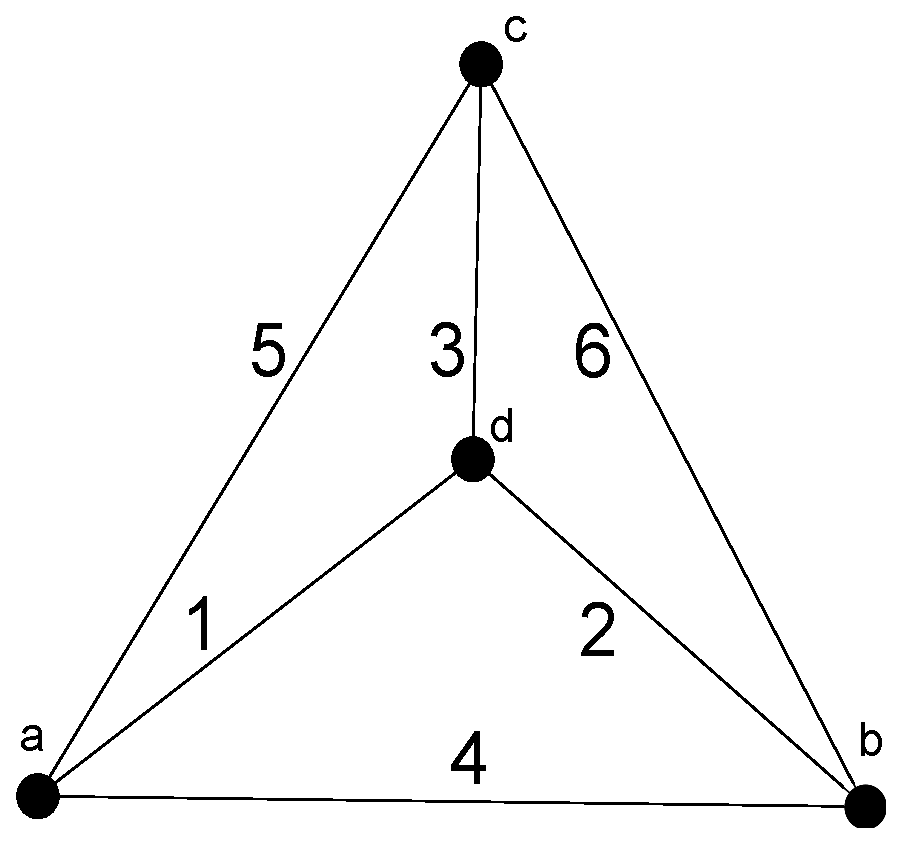
\includegraphics[width=6cm]{Test1/Problem1/tetrahedron.eps}
                \label{fig:tetrahedron}
            \end{figure}
            
            Now lets think what could happen if $M_3[A]$. For $M_3[A]$, we have the circuits 
            $\{1, 4, 5, 6\}, \{2, 4, 5, 6\}, \{3, 4, 5, 6\}$. Take any two of them, lets say
            $\{1, 4, 5, 6\}, \{2, 4, 5, 6\}$, they have three edges in common $\{4,5,6\}$. \pn
            
            If there is a graphic mathroid isomorphic to $M_3[A]$, $\{4,5,6\}$ defines three edges of a 
            $4$-cycle, that is, a $3$-trajectory. In any $3$-trajectory we will find $4$ vertices, so the fourth 
            edge is already determined by two of those vertices (the start vertex and the last vertex), but in this case 
            we have that $\{1, 4, 5, 6\}$, $\{2, 4, 5, 6\}$ are both $4$-cycles over the same set of vertices, 
            and so $1$ and $2$ have exactly the same two vertices, that is, they are parallel. But in [\ref{t1:p1}.\ref{t1:p1i}]
            we saw that $M_3[A]$ has no parallel columns. So this is a contradiction.
        
        \item\label{t1:p1iii}
            We are going to give a matrix $B$ over $GF(3)$ such that $M_3[B]$ isomorfic to $M_2[A]$.\pn
            
            We are going to take the incidence matrix for the graphic representation [\ref{fig:tetrahedron}], and
            choose one ``1'' from each column and change it by ``-1''. What we are doing is giving a orientation
            to each of the edges. So, if a cycle is such that each edge has exactly outdegree 1 and indegree 1, is
            easy to see that the sum of the respective columns will be the zero vector (each 1 will have exactly one -1 in
            its same row).\pn
            
            But lets remember that we are taking linear combination over $GF(3)$, that is, we can take a column, 
            its negative, or take the zero vector instead. So, if we have a cycle, not necessarily ``well-oriented'',
            we can give it a ``good-orientation'' by multiplying its edges by -1 or 1 such way that each vertex 
            has outdegree 1 and indegree 1. If we sum them, we will get the zero vector, and givin a ``good-orientation'' is
            no other thing than finding a linear combination that sums up 0.\pn
            
            So, let B be the matrix
            $$\bordermatrix{
                    &   1   &   2   &   3   &   4   &   5   &   6   \cr
                a   &   -1  &   0   &   0   &   1   &   -1  &   0   \cr
                b   &   0   &   -1  &   0   &   -1  &   0   &   1   \cr
                c   &   0   &   0   &   -1  &   0   &   1   &   -1  \cr
                d   &   1   &   1   &   1   &   0   &   0   &   0   \cr
            }$$
            
            By the explanation just given, each circuit in $M_2[A]$ is a circuit in $M_3[B]$ (note that we used the same 
            labels in both matrices so the subsets of labels can have the same representation).\pn
            
            Also, note that if you choose a subset of edges such that you have leaves, the row for any leaf cannot be
            zero under any linear combination unless you multiply it by 0. Having said these, is easy to see that
            the subsets of columns representing forests are independent.\pn
            
            Now, lets suppose there is a matrix $C$ such that $M_2[C]$ is isomorphic to $M_3[A]$. Again, lets suppose that 
            the labels are the same in both matrices. Then, you must have that the subsets of columns $\{1, 4, 5, 6\}$ and 
            $\{2, 4, 5, 6\}$ are circuts. So, the sum of the columns 4, 5, 6 and 1 must be the zero vector, that is the column 1
            is equal to the sum of the columns 4, 5 and 6. But the same occurs with the other circuit, the sum of columns
            4, 5, 6 and 2 must be zero, so the colun 2 is equal to the sum of the columns 4, 5 and 6. Then we have that the
            columns 1 and 2 must be the equal. That is, the columns 1 and 2 are parallel. Which is a contradiction to what we
            proved in [\ref{t1:p1}.\ref{t1:p1i}].
            
        \end{enumerate}
\end{proof}
        \clearpage

    \section{Oxley, Section 1.1, Problem 7}
        \prob
{
    Let $M_1$ and $M_2$ be matroids on disjoint sets $E_1$ and $E_2$ and with independent sets
    $\I_1$ and $\I_2$ respectively. Let $E = E_1 \cup E_2$ and 
    $\I = \{ I_1 \cup I_2 : I_1 \in \I_1, I_2 \in \I_2\}$. Prove that $(E, \I)$ is a
    matroid.
}

\begin{proof}
    Lets see that $(E, \c{I})$ satisfies $I1, I2$ and $I3$.\pn
        
    \begin{enumerate}
        \item[(I1)]
            $\emptyset \in \I$. This is clear, $\emptyset \in \I(M_1)$ and $\emptyset \in \I(M_1)$, so 
            $\emptyset = \emptyset \cup \emptyset \in \I$.\pn
            
        \item[(I2)]
            If $I \in \I$, $J \subset I$ then $J \in \I$. $I \in \I$ means that there are $I_1 \in \I_1$
            and $I_2 \in \I_2$ such that $I = I_1 \cup I_2$. Given that $J \subset I$ it is clear that
            $J = J \cap I = J \cap (I_1 \cup I_2) = (J \cap I_1) \cup (J \cap I_2)$. We have that $(J \cap I_1) 
            \subset I_1$ and $(J \cap I_2) \subset I_2$, given that $M_1$ and $M_2$
            are matroids, then $(J \cap I_1) \in \I_1$ and $(J \cap I_2) \in \I_2$. 
            Then $J = (J \cap I_1) \cup (J \cap I_2) \in \I$.\pn
            
        \item[(I3)] 
            If $I, J \in \I$, $|J| < |I|$ then there exists $x \in I \setminus J$ such that $J \cup \{x\} \in \I$.
            By hypotesis, there are $I_1, J_1 \in \I_1$ and $I_2, J_2 \in \I_2$ such that $I = I_1 \cup I_2$ and $J = J_1 \cup J_2$.
            Then $|J| = |J_1| + |J_2| <  |I_1| + |I_2| = |I|$. Then there must be that $|J_1| < |I_1|$ or
            that $|J_2| < |I_2|$. Withtout loss of generality, lets say that $|J_1| < |I_1|$, as $M_1$ is a matroid,
            then, there exists $x \in I_1 \setminus J_1$ such that $J_1 \cup \{x\} \in \I_1$. Then, $x \in I$ and 
            $J \cup \{x\} = (J_1 \cup \{ x \}) \cup J_2 \in \I$. And we are done.\pn
            
    \end{enumerate}
\end{proof}
        \clearpage
    \section{Oxley, Section 1.1, Problem 9}
        \prob
{
    Let $M_1$ and $M_2$ be matroids on a set $E$. Give an example to show that
    $(E, \I(M_1) \cap \I(M_2))$ need not be a matroid.
}

\begin{proof}
    Let $E = \{a, b, c\}$.
    
    Let $\I(M_1) = \{ \{a, b\}, \{a, c\}, \{a\}, \{b\}, \{c\}, \emptyset \}$
    Lets check that this is a matroid. It hass the empty set, given any set, any of its subests is independent.
    To see that the independence augmentation axiom (if $I, J \in \I$ and $|J| < |I|$ then there exists
    $x \in I \setminus J$ such that $J \cup \{x\}  \in \I$), I will give you a table, where the first row is for the
    set $I$, the second for $J$ and the third one for $x$.\pn
    
    \begin{center}
        \begin{tabular}{ | p{1cm} | p{1cm} | p{1cm} |}
            \hline $I$          & $J$           &   $x$ \\ \hline
            \hline $\{a, b\}$   & $\{a\}$       &  b    \\
            \hline $\{a, b\}$   & $\{b\}$       &  a    \\
            \hline $\{a, b\}$   & $\{c\}$       &  a    \\
            \hline $\{a, b\}$   & $\emptyset$   &  a    \\
            \hline $\{a, c\}$   & $\{a\}$       &  c    \\
            \hline $\{a, c\}$   & $\{b\}$       &  a    \\
            \hline $\{a, c\}$   & $\{c\}$       &  a    \\
            \hline $\{a, c\}$   & $\emptyset$   &  a    \\
            \hline $\{a\}$      & $\emptyset$   &  a    \\
            \hline $\{b\}$      & $\emptyset$   &  b    \\
            \hline $\{c\}$      & $\emptyset$   &  c    \\ \hline
        \end{tabular}    
    \end{center}
    
    So $(E, \I(M_1))$ is a matroid.\pn
        
    Now, let $\I(M_2) = \{ \{a, b\}, \{b, c\}, \{a\}, \{b\}, \{c\}, \emptyset \}$, to see that $(E, \I(M_2))$ 
    the first two axioms can be justified just as above, and just below is the table to check the augmentation axiom.\pn
    
   \begin{center}
        \begin{tabular}{ | p{1cm} | p{1cm} | p{1cm} |}
            \hline $I$          & $J$           &   $x$ \\ \hline
            \hline $\{a, b\}$   & $\{a\}$       &  b    \\
            \hline $\{a, b\}$   & $\{b\}$       &  a    \\
            \hline $\{a, b\}$   & $\{c\}$       &  b    \\
            \hline $\{a, b\}$   & $\emptyset$   &  a    \\
            \hline $\{b, c\}$   & $\{a\}$       &  b    \\
            \hline $\{b, c\}$   & $\{b\}$       &  c    \\
            \hline $\{b, c\}$   & $\{c\}$       &  b    \\
            \hline $\{b, c\}$   & $\emptyset$   &  b    \\
            \hline $\{a\}$      & $\emptyset$   &  a    \\
            \hline $\{b\}$      & $\emptyset$   &  b    \\
            \hline $\{c\}$      & $\emptyset$   &  c    \\ \hline
        \end{tabular}    
    \end{center}
    
    So $(E, \I(M_2))$ is also a matroid.\pn
    
    Then $\I' = \I(M_1) \cap \I(M_2) = \{ \{a, b\}, \{a\}, \{b\}, \{c\}, \emptyset \}$ cannot be an independet set for $E$. 
    It satisfies (I1) and (I2), but not I3 since $\{a, b\}, \{c\} \in \I'$, and $|\{c\}| < |\{a, b\}|$ but 
    $\{c\} \cup \{a\} \not\in \I'$ and $\{c\} \cup \{b\} \not\in \I'$.
\end{proof}
        \clearpage

    \section{Oxley, Section 1.2, Problem 1}
        \prob
{
    Prove that $\B$ is the collection of bases of a matroid on 
    $E$ if and only if $\B$ satisfies (B1) and the following two conditions:
    
    \begin{itemize}
        \item[(B2)'] If $B_1, B_2 \in \B$ and $e \in B_1$, then there is an element $f$ of
                        $B_2$ such that $(B_1 \setminus \{e\}) \cup \{f\} \in \B$.
                        
        \item[(B3)] If $B_1, B_2 \in \B$ and $B_1 \subset B_2$, then $B_1 = B_2$.
    \end{itemize}
}

\begin{proof}
    Suppose that $\B$ is the collection of bases of a matroid.
    
    Then, it satisfies (B1) and.
\end{proof}
        \clearpage

    \section{Oxley, Section 1.2, Problem 6}
        \prob
{
    Suppose $B$ is a basis of a matroid $M$, $f \in E(M)$ and $e \in E(M) \setminus B$.
    Prove that $(B\cup \{e\}) \setminus \{ f \}$ is a basis of $M$ if and only if $f \in C(e, B)$.
}
\begin{proof}$\,$\pn
    The \textbf{sufficiency} is not true.\pn
    
    Counterexample. Let $E = \{1, 2, 3\}$, and let $\I$ be the power set of $\{1, 2\}$ which trivialy
    satisfies (I1), (I2) and (I3). And $M$ the matroid $(E, \I)$.\pn
    
    $B = \{1, 2\}$ is a basis (and the only one) of $M$.
    
    $f = 2$ is in $E$.
    
    $e = 3$ is in $E \setminus B$.
    
    $f \in \{1, 2, 3\} = C(e, B)$.
    
    But $(B \cup \{ e \}) \setminus \{ f \} = \{1, 3\} \not\in \B$.\pn
    
    \textbf{Necessity}
    
\end{proof}
        \clearpage

    \section{Oxley, Section 1.3, Problem 4}
        \prob
{
    Prove that a matroid $M$ is uniform if and only if it has no circuits of 
    size less than $r(M) + 1$.
}
\begin{proof}
	Suppose that $M$ is a uniform matroid $U_{m, n}$, then $r(M) = m$ by definition.
    Moreover, any $A \subset E(M)$ such that $|A| < m$ will be subset of some basis and
    therefore independent. Then if there is any circuit $C$, it must have size greater
    than $m$, that is $r(C) \geq m + 1 = r(M) + 1$.\pn

    \textbf{Necessity}\pn
    
    Suppose now that $M$ is such that it has no circuits of size less than $r(M) + 1$.
    Then, for any $A \subset E(M)$ with $|A| \leq r(M)$ it must be independent, if not,
    then $A$ should contain a circuit, but any circuit has size at least $r(M) + 1$.\pn
    
    Then $M$ must be isomorphic to an uniform matroid $U_{r(M), |E(M)|}$.
\end{proof}
        \clearpage

    \section{Oxley, Section 1.3, Problem 5}
        \prob
{   $\,$\pn
    \begin{enumerate}[label=(\roman*)]
        \item   Characterize paving matroids in terms of their collection of 
                independent sets and in terms of their collections of bases.
        
        \item   Characterize uniform matroids in terms of their collections of 
                circuits.
    \end{enumerate}
}
\begin{proof}
    $\;$\pn
    \begin{enumerate}[label=(\roman*)]
        \item   Let $M$ be a matroid. $\B$ its collection of bases and $\I$ its collection
                of independent sets.\pn
                
                $M$ is a paving matroid if and only if for every $A \subset E(M)$ with
                $|A| < r(M)$ there exists $B \in \B$ such that $A \subset B$.\pn
                
                As $M$ is matroid, by $I2$, this is exactly the same as saying:\pn
                
                $M$ is a paving matroid if and only if for every $A \subset E(M)$ with
                $|A| < r(M)$, $A \in \I$.\pn
                
                \begin{proof}
                    If $M$ is paving, by definition of paving matroid, any $A \in E(M)$ such
                    that $|A| < r(M)$ then, $A \in \I$ (and therefore, there is some $B \in \B$
                    such that $A \subset B$).\pn
                    
                    If $M$ is a matroid such that for every $A \subset E(M)$ with
                    $|A| \leq r(M)$ there exists $B \in \B$ such that $A \subset B$ (and 
                    therefore, $A \in \I$). Then, suppose that $C$ is a circuit of $M$. 
                    If $|C| < r(M)$, then there would be some $B \in \B$ such that 
                    $C \subset B$, but then $C \in \I$, which is a contradiction and therefore 
                    $|C| \geq r(M)$. That is, $M$ is paving.\pn
                \end{proof}
                
        \item   A matroid $M$ is uniform if and only if it has no circuits of size less than 
               $r(M) + 1$.
            
                \begin{proof}
                    See (\ref{t1:p6})
                \end{proof}
    \end{enumerate}
\end{proof}
        \clearpage

    \section{Oxley, Section 1.4, Problem 2}
        \prob
{
    Show that a subset $X$ of a matroid is a basis if and only if $X$ is both independent and spanning.
}
\begin{proof}
    $\,$\pn
    \textbf{Sufficiency}\pn

    If $X$ is a basis of a matroid $M$, then by definition of basis, it is independent. Also, as $X$ is
    basis, then $r(X) = r(X \cup x)$ for any $x \in E(M)$ and, therefore, $cl(X) = E(M)$, that is, $X$ is spanning.\pn
    
    \textbf{Necessity}\pn
    
    Suppose that $X$ is both independent and spanning. As $X$ is spanning, then $r(X) = r(M)$, that is, for any $B \in \B(M)$,  
    $|X| \geq r(X) = r(B) = |B|$. On the other hand, $X \in \I(M)$ so, for any $B \in \B(M)$, $|X| \leq |B|$. We have then that
    $|B| \leq |X| \leq |B|$, that is $|B| = |X|$ for any $\B(M)$ and therefore, $X$ is a basis.
    
\end{proof}
        \clearpage

    \section{Oxley, Section 1.4, Problem 6}
        \prob
{
    Prove that statments (a)-(g) below are equivalent for an element $e$ of a matroid $M$:
    \begin{enumerate}[label=(\alph*)]
        \item $e$ is in every basis.
        \item $e$ is in no circuits.
        \item If $X \subseteq E(M)$ and $e \in cl(X)$, then $e \in X$.
        \item $r(E(M) \setminus \{e\}) = r(E(M)) - 1$.
        \item $E(M) \setminus \{e\}$ is a flat.
        \item $E(M) \setminus \{e\}$ is a hyperplane.
        \item If $I$ is an independent set, then so is $I \subset e$.
    \end{enumerate}
}
\begin{proof}
\end{proof}
        \clearpage

    \section{Oxley, Section 1.6, Problem 1}
        \prob
{
    Show the following:
    \begin{enumerate}[label=(\roman*)]
        \item   All uniform matroids are transversal.
        \item   A transversal matroid need not be graphic.
        \item   A paving matroid need not be transversal.
    \end{enumerate}
}
\begin{proof}
\end{proof}
        \clearpage

    \section{Oxley, Section 1.6, Problem 3}
        \prob
{
    Let $S = \{1, 2, \dots, 6\}$ and $\c{A} = \{A_1, A_2, A_3\}$ where $A_1 = \{1, 2, 3\}$
    $A_2 = \{2, 3, 4\}$, and $A_3 = \{4, 5, 6\}$.
    \begin{enumerate}[label=(\roman*)]
        \item   Find $\Delta[\c{A}]$.
        \item   Give a geometric representation for $M[\c{A}]$.
    \end{enumerate}
}
\begin{proof}$\,$\pn
    \begin{enumerate}
        \item   Graphic representation for for $\Delta[\c{A}]$

                \begin{figure}[H]%
                    \centering
                    \caption{}%
                    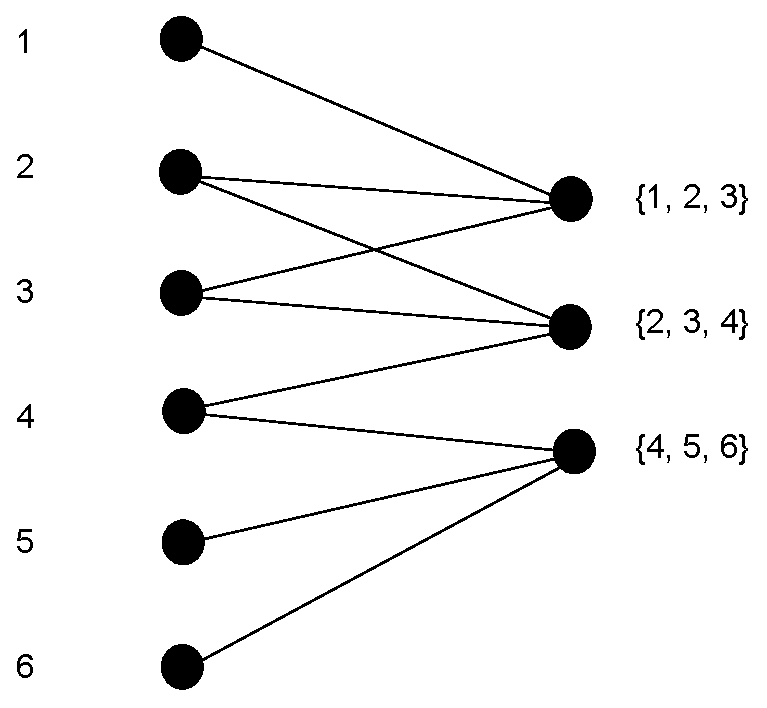
\includegraphics[width=6cm]{Test1/Problem11/deltaA.eps}
                \end{figure}
        
        \item   Geometric representation for $M[\c{A}]$
    \end{enumerate}

\end{proof}
        \clearpage

    \section{Oxley, Section 1.6, Problem 4}
        \prob
{
    Characterize the circuits of $M[\c{A}]$ in terms of the bipartite graph $G = \Delta[\c{A}]$.
}
\begin{proof}
    Lets remember that $G = \Delta[\c{A}]$ is a bipartite graph with partition $(S, \c{A})$ and that
    in terms of transversal matroids, a subset $T \subset S$ is independent if there is an injection
    $\phi : T \rightarrow \c{A}$ such that $(t, \phi(t))$ is and edge for every $t \in T$.\pn
    
    Halls theorem states that a susbset $T \subset S$ is independent if and only if $|U| \leq |N_G(U)|$.
    For every $U \subset T$.\pn
    
    That is, a subset $T \subset S$ is dependent if and only if there is $U \subset T$ such that $|U| > |N_G(U)|$. 
    We are looking for subsets $T$ that satisfies this condition and that are minimal.\pn
    
    If there is $U \subsetneq T$ such that  $|U| > |N_G(U)|$, then $T$ can not be minimal.
    
    Then $T$ must has the property $|T| > |N_G(T)|$ (we will refer to this property as the
    $(*)$-property) and its minimal.\pn

    Then, $T$ is a circuit if and only if it is has the $(*)$-property and its minimal with such condition.
    
    We can learn a little more about these $T$'s. Lets check what happen if the graph induced by $T$ has at least 
    $2$ connected components. Lets call $T_1$ and $T_2$ such that $T_1$ induces one connected component and $T_2 = T \setminus T_1$.
    Notice that $N_G(T_1) \cap N_G(T_2) = \emptyset$, and then $|N_G(T)| = |N_G(T_1)| + |N_G(T_2)|$. 
    As $|T| = |T_1| + |T_2| > |N_G(T_1) | + |N_G(T_2)| = |N_G(T)|$ 
    it must be that either $|T_1| > |N_G(T_1)|$ or $|T_2| > |N_G(T_2)|$, without loss of generality, 
    if the first one is true, then at least $T_1$ is smaller than $T$ and then $T$ is not minimal. 
    Then the graph induced by $T$ must     be connected.\pn
     
    %$P$ is switching from $T$ to $\c{A}$. $P$ starts in $\c{A}$, then you can 
    %enumerate the edges of $P$ starting from a start edge and giving the next number to the only edge that is connected to the already numbered
    %edges, if you take the odd edges, as $P$ is spaning, then you can cover all of $T$, which is a contradiction because $T$ had
    %the $(*)$-property. Then $P$ has not start vertex in $\c{A}$, with the same procedure we can show that $P$ has no end vertex in $\c{A}$.\pn
    %
    %Then any $P$ must start and end in $T$, and then, $P$ is even. Notice then, that $|T| = |N_G(T)| + 1$. 
    %If you remove the start (or end) vertex $v$, you get a subpath that starts (ends) in $\c{A}$ and then it covers all of $T \setminus \{v\}$ with 
    %a matching as seen above. If you remove any other vertex $v$ from $T$ different from the start and end vertices, then you make two paths that 
    %start (end) in $\c{A}$ and then $T \setminus \{v\}$ is covered by a matching. That is, if you remove any vertex, you can have a matching that 
    %covers the vertices from $T$ left, that is,if you remove any vertex the $(*)$-property is loss \pn 
    %
    %Then we can characterize the circuits of $M[\c{A}]$
\end{proof}
        \clearpage

    %\section{Oxley, Section 1.7, Problem 5}
        %MISSING
				%\prob
{
    Prove that a finite lattice $\c{L}$ is semimodular if, for all $x$, $y$ in $\c{L}$, the following condition holds:\pn
    \;\;\textsc{If both $x$ and $y$ cover $x \wedge y$, then $x \vee y$ covers both $x$ and $y$}.
}
\begin{proof}
\end{proof}
        %\clearpage

    \section{Oxley, Section 1.8, Problem 1}
        \prob
{
    \begin{enumerate}[label=(\roman*)]
        \item   Find a maximum-weight spanning tree of the graph in the next figure. Is this the unique such tree?
                \begin{center}
                    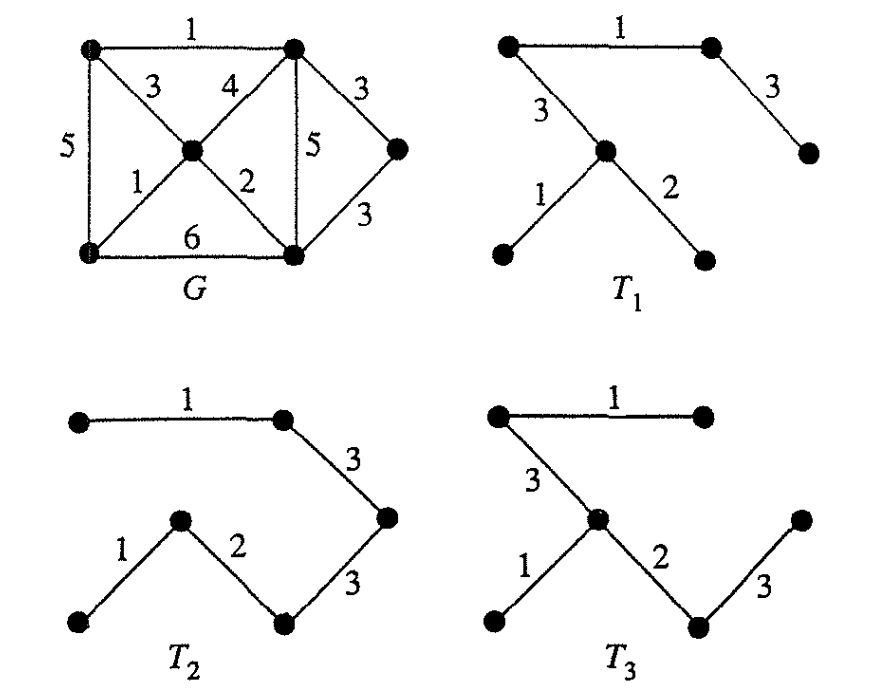
\includegraphics[width=8cm]{Test1/Problem14/Figure-i.png}
                \end{center}
                
        \item   Find all maximum-weight spanning trees and all minimum-weight spanning trees of the graph in the next
                figure, where the edge labels are interpreted as weights.
                \begin{center}
                    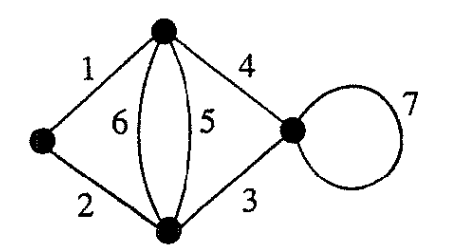
\includegraphics[width=4cm]{Test1/Problem14/Figure-ii.png}
                \end{center}
    \end{enumerate}
}
\begin{proof}
\begin{enumerate}
	\item 
            There are only 2 maximum-weight spanning trees of the graph. I have ilustrated what will greedy do step by step,
            and with all possible desicions being made.
            \begin{center}
                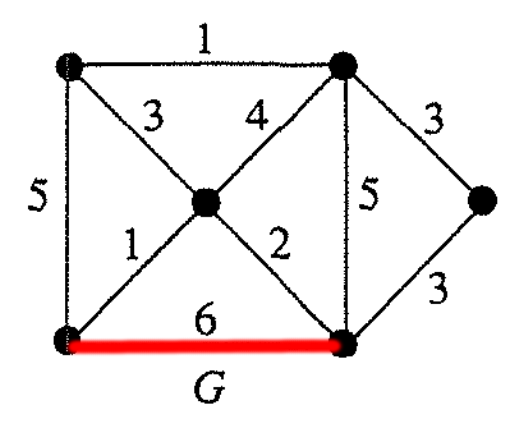
\includegraphics[width=4cm]{Test1/Problem14/Fig-i-1.png}
            \end{center}
            
            \begin{center}
                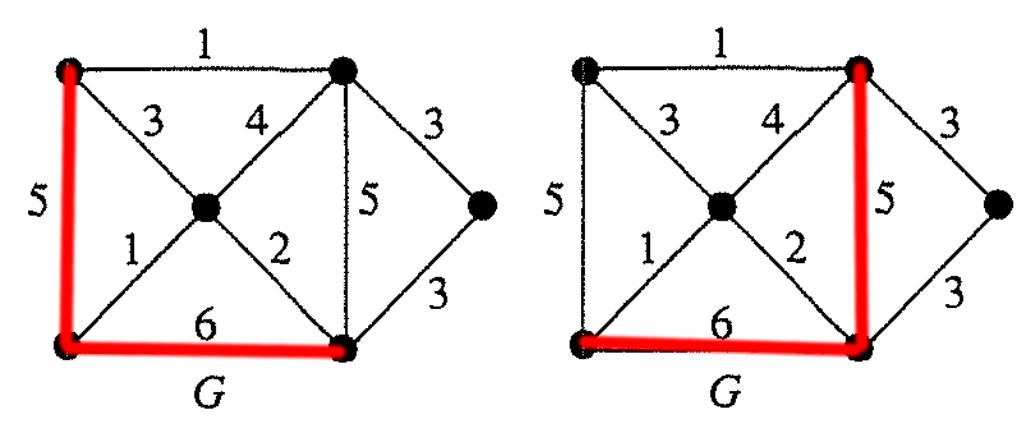
\includegraphics[width=8cm]{Test1/Problem14/Fig-i-2.png}
            \end{center}
            
            \begin{center}
                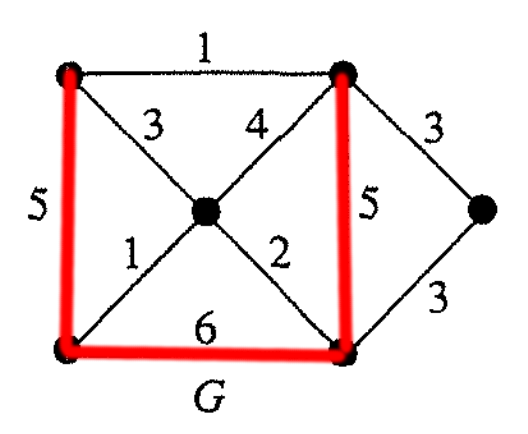
\includegraphics[width=4cm]{Test1/Problem14/Fig-i-3.png}
            \end{center}
            
            \begin{center}
                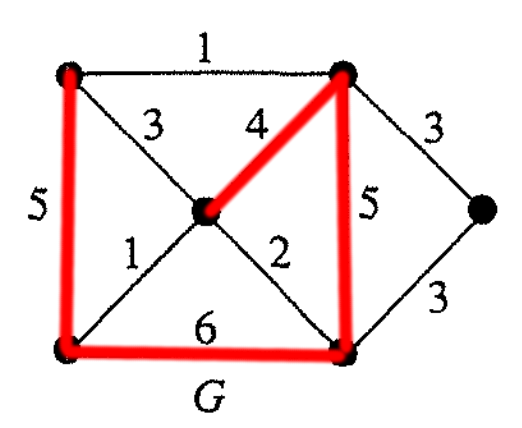
\includegraphics[width=4cm]{Test1/Problem14/Fig-i-4.png}
            \end{center}
            
            \begin{center}
                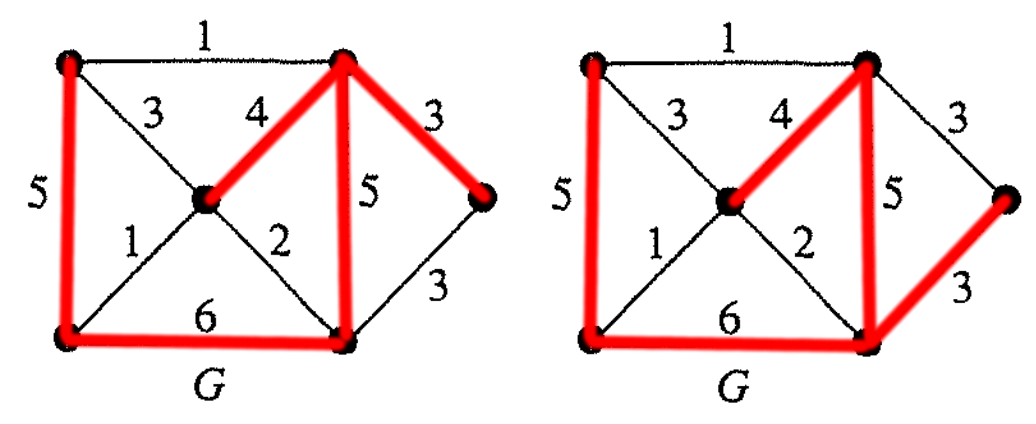
\includegraphics[width=8cm]{Test1/Problem14/Fig-i-5.png}
            \end{center}
    \item
            As the weight function is injective, the maximum-weight and minimum-weight spanning trees are unique.\pn
            
            Here is again an ilustration of what greedy would do in both scenarios.\pn
            
            Maximum-weight:\pn
            
            \begin{center}
                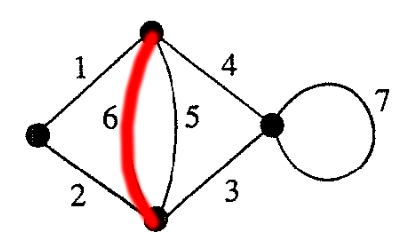
\includegraphics[width=5cm]{Test1/Problem14/Fig-ii-a-1.png}
            \end{center}
            
            \begin{center}
                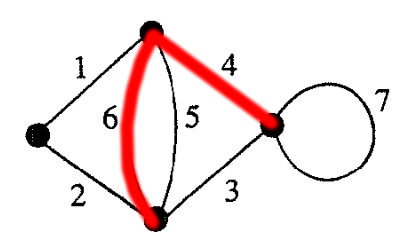
\includegraphics[width=5cm]{Test1/Problem14/Fig-ii-a-2.png}
            \end{center}
            
            \begin{center}
                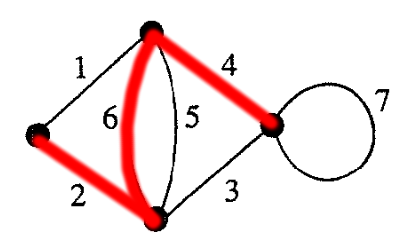
\includegraphics[width=5cm]{Test1/Problem14/Fig-ii-a-3.png}
            \end{center}     
                
            Minimum-weight:\pn
            
            \begin{center}
                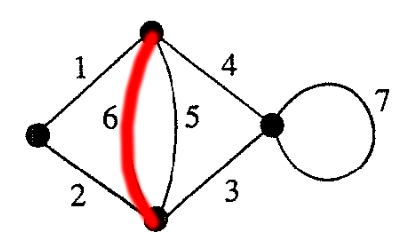
\includegraphics[width=5cm]{Test1/Problem14/Fig-ii-a-1.png}
            \end{center}
            
            \begin{center}
                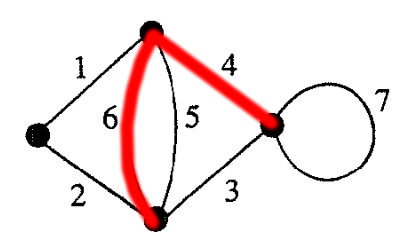
\includegraphics[width=5cm]{Test1/Problem14/Fig-ii-a-2.png}
            \end{center}
            
            \begin{center}
                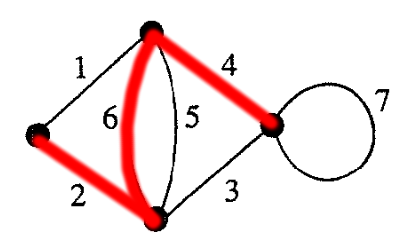
\includegraphics[width=5cm]{Test1/Problem14/Fig-ii-a-3.png}
            \end{center}
\end{enumerate}
\end{proof}
        \clearpage

    \section{Oxley, Section 1.8, Problem 4}
        \prob
{
    Let $M$ be a matroid and $\omega: E(M) \rightarrow \R$ be a one-to-one function. 
    Prove that $M$ has a unique basis of maximum weight.
}
\begin{proof}
    Let $B$ be a maximum-weight basis found using greedy. Suppose that there is another basis $B'$ with maximum-weight also and
    suppose that they are different.\pn
    
    Let $e \in B' \setminus B$ of minimum-weight (it exists because $\omega$ is one-to-one), and then, there exists $f \in B \setminus B'$ such that
    $(B' \setminus \{e\}) \cup  \{f\}$ is basis. We can choose such $f$ of maximum weight. If $\omega(e) < \omega(f)$ then we have increased the 
    weight of $B'$, which is a contradiction. If $\omega(f) < \omega(e)$ we can change the roles of $B$ and $B'$ and get the same contradiction.\pn
    
    So, there is no other basis $B'$ with maximum-weight and different from $B$.
\end{proof}
        \clearpage

\chapter{Second Test}
    \section{Oxley, Section 2.1, Problem 1}
        \prob{
    Find each of the following:
    \begin{enumerate}[label=(\roman*)]
        \item all self-dual uniform matroids;
        \item all identically self-duall uniform matroids;
        \item all self-dual graphic matroids on six or fewer elements;
        \item all identically self-dual graphic matroids on six or fewer elements;
        \item an infinite family of simple graphic self-dual matroids.
    \end{enumerate}
}
\begin{proof}$\,$\pn
    \begin{enumerate}[label=(\roman*)]
        \item 
            Let $U_{n,m}$ be an uniform matroid.\pn
            
            Lets asume that it is self-dual. As
            any basis $B$ for $U_{n,m}$ has size $n$, if it is going to be self-dual,
            then its complement must have size $n$ as well. This means that $m = 2n$.\pn
            
            Now lets suppose that $m = 2n$. So, any subset of size $n$ is a basis for $U_{n,m}$,
            but it is also true that any subset of size $n$ is the complement of another subset
            of size $n$ and then, any basis is the complement of another basis. Then $U_{n,m}$ is
            not only self-dual, but also identically self-dual.
        \item 
            Just as we saw above, if an uniform matroid is self-dual, then it is identically self-dual, and
            an uniform matroid $U_{n,m}$ is self-dual if and only if $m = 2n$.
            
        \item 
            It is clear that if a matroid is to be self-dual, then its size must be two times
            the size of any of its basis (any forest that is not contained in any other forest). 
            This means that there are only self-dual graphic matroids with an even number of edges. \pn
            
            Lemma 2.3.7 from~\cite{Oxley} stays that if $G^*$ is a geometric dual of the planar graph $G$, then
            $M(G^*) \cong M^*(G)$. In particular for self-dual matroids we will have that $M(G^*) \cong M^*(G) \cong M(G)$.
            
            From now on we will use this fact to look for the remaining self-dual matroids. As the maximum size of these matroids
            is $6$ and $K_4$ is a complete planar graph with 6 edges, then every one of the matroids will have a planar representation. 
            And the previously mentioned lemma will let us work with graph representations instead of a complicated structure of 
            subsets and its intersections.\pn
            
            Also, notice that if $G$ is a planar graph. And $H = G \cup G^*$, then $M(H)$ is self-dual. The only
            trick is to send $M(G)$ to $M(G)$ in the dual and $M(G^*)$ to $M(G^*)$ in the dual.\pn
            
            Considering this. We will try to find self-duality through blocks (2-connected maximal subgraphs) when it is possible.
            Also, the drawings will be done thinking of these, we are going to separate in as many blocks as possible, given that
            it will not affect the resultant matroid.\pn
            
            We will try to order our analysis by the size of the maximum cycle contained in a graph or its dual matroid. And for this
            remember that the dual of a $n$-cycle is a set of $n$ edges all of them parallel to each other.\pn            
            
            \textbf{2 edges}:\pn
                \begin{itemize}
                    \item \textbf{No cycles.}
                        There is no such graph. If a graph has no cycles, then its dual contains only loops (which are cycles).
                        This will happen in any of the other graphs so we are not going to list this case anymore.
                    
                    \item \textbf{Cycles of size at most 1.}
                        If there has to be a loop, then it has to be an edge that is not a loop. The loop will be maped to the dual of
                        the edge that is not a loop and viceversa. This one is not identically self-dual. 
                        
                        \begin{figure}[H]
                            \begin{center}
                            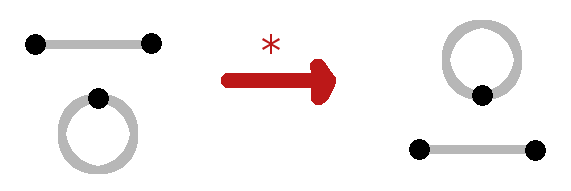
\includegraphics[width=5cm]{Test2/Problem1/1_0.png}
                            \end{center}
                            \caption{self-dual graphic matroid representation}
                            \label{t2:p1_1_0.png}  
                        \end{figure}\pn
                        
                    \item \textbf{Cycles of size at most 2.}
                        There is only one way to get a cycle of size two with two edges, and it is easy to see that it has not only
                        a self-dual matroid but an identically auto-dual matroid.
                        
                        \begin{figure}[H]
                            \begin{center}
                            
\includegraphics[width=5cm]{Test2/Problem1/2.png}
                            \caption{identically self-dual graphic matroid representation}
                            \label{t2:p1_2.png}
                            \end{center}                        
                        \end{figure}\pn
                \end{itemize}
                  
                There cannot be larger cycles with only 3 edges.\pn
            \textbf{4 edges}:\pn
            
                \begin{itemize}
                   \item \textbf{Cycles of size at most 1.}
                        Again. For every loop ther must be an edge that is not a loop. And for every edge that is not a loop there 
                        must be a loop. So the only posibility left is to have two loops and two edges that are not loops.
                        
                        \begin{figure}[H]
                            \begin{center}
                            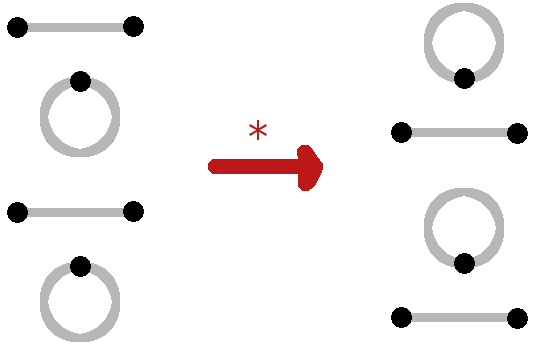
\includegraphics[width=5cm]{Test2/Problem1/1_0-1_0.png}
                            \end{center}                        
                        \end{figure}\pn
                        
                   \item \textbf{Cycles of size at most 2.}
                        If we have a block as in \ref{t2:p1_2.png}, then, under the matroid isomorphisim are two posibilities,
                        that such block is mapped into itself, or that it is mapped into another block.
                        
                        If it is mapped into another block, then the other block must be essentialy the same graph and then
                        whe have something like
                        \begin{figure}[H]
                            \begin{center}
                            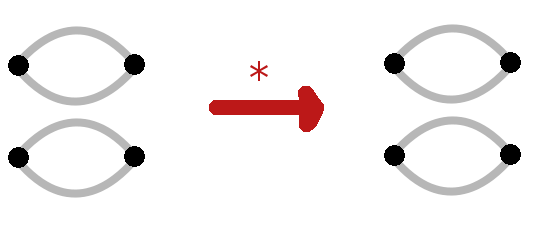
\includegraphics[width=5cm]{Test2/Problem1/2-2.png}
                            \end{center}                            
                            \caption{identically self-dual graphic matroid representation}
                            \label{t2:p1_2-2.png}                        
                        \end{figure}\pn
                        
                        (Notice that this will result in an identically self-dual matroid also. Every forest is a pair of
                        non-parallel edges, and its complement is also a pair of non-parallel edges.)\pn
                        
                        If the first block is mapped into itself, then the other block must be mapped into itself also.
                        Then the other block must be a representation of a self-dual matroid on 2 edges. And then, there are
                        two posibilities. If the other block is like in \ref{t2:p1_2.png}, then we will obtain again 
                        \ref{t2:p1_2-2.png}. If the other block is like \ref{t2:p1_1_0.png} then we will obtain something like
                        \begin{figure}[H]
                            \begin{center}
                            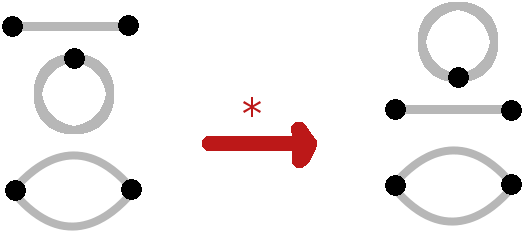
\includegraphics[width=5cm]{Test2/Problem1/2-1_0.png}
                            \end{center}                            
                            \caption{self-dual graphic matroid representation}
                            \label{t2:p1_2-1_0.png}                        
                        \end{figure}\pn
                        
                        (Notice that this could not be identically self-dual. As it has loops, any loop will be in a cobasis, but no
                        basis contains loops.)\pn
                        
                    \item \textbf{Cycles of size at most 3.}
                        A graph that will represent a self-dual matroid and that has a 3-cycle and at most 4 edges, must have at most
                        one block. Otherwise, on block must be the triangle, but a triangle is not self-dual and could not be mapped 
                        in the other block that only could have 1 edge.\pn
                        
                        This gives us essentially only one opportunity. A triangle adding a parallel edge to one of its edges.
                        An isomorphism would be sending the simple edges to the parallel edges and the parallel edges to the simple 
                        edges. The two simple edges form a set that intersects any of the basis of the matroid, so it is a cocircuit. 
                        The proposed isomorphism send that cocircuit to a circuit in the original matroid. The two parallel edges along 
                        with any of the simple edges form another set that intersects any of the basis of the original matroid, so it 
                        is another cocircuit in the dual matroid. Those edges are sent to a triangle in the original matroid. There 
                        are two of these cocircuits and each one is sent two one of the two possible triangles in the original matroid.
                        Any basis formed for a simple edge and one of the two parallel edges has as complement the other simple edge 
                        and the other parallel edge, and under the proposed isomorphism any of such basis are sent to other of the 
                        same type. The only other basis that is left is the one that consits of the two simple edges, and they are 
                        sent to the pair of parallel edges, which is independent in the dual matroid. We have proved so far that this 
                        isomorphism sends any of the basis in the original matroid to a basis in the dual matroid and any cocircuit 
                        to a circuit in the original matroid. Then such isomorphism is a matroid isomorphism between the graphic matroid 
                        and its dual.\pn
                        
                        \begin{figure}[H]
                            \begin{center}
                            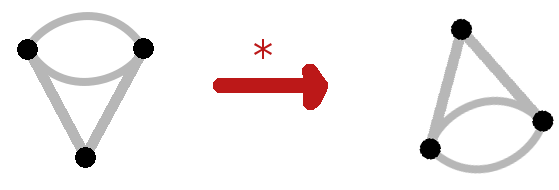
\includegraphics[width=5cm]{Test2/Problem1/4.png}
                            \end{center}                            
                            \caption{self-dual graphic matroid representation}
                            \label{t2:p1_4.png}                        
                        \end{figure}\pn
                        
                        This could not be identically self-dual as it has a cobasis that contains parallel edges.
                        
                    \item \textbf{Cycles of size at most 4.}
                        There is none, as the only cycle of size 4 has 4 edges, and as the 4-cycle is not self-dual, there cannot be
                        self-dual matroids with 4-elements and 4-cycles.
                \end{itemize}
    
                There cannot be larger cycles with only 4 edges.\pn
            \textbf{6 edges}:\pn
            MISSING!
        \item 
            Any graph on six or fewer elements obtained from a forest adding a parallel edge to each edge in the forest.
            We have proved this in the last part, indicating which of the self-dual matroids are identically self-dual or non-identically self-dual.
            
        \item 
            Any wheel. Proof in [\ref{p11}]
    \end{enumerate}
\end{proof}
        \clearpage

    \section{Oxley, Section 2.1, Problem 2}
        \prob{
    Let $M$ be a matroid. Show that $M*$ has two disjoint circuits if and only if $M$ has two hyperplanes whose union is $E(M)$.
}
\begin{proof}
\end{proof}
        \clearpage

    \section{Oxley, Section 2.1, Problem 6}
        \prob
{
    Let $e$ and $f$ be distinct elements of a matroid. Prove that every circuit containing $e$ also contains $f$ if and only if 
    $\{e\}$ or $\{e, f\}$ is a cocircuit.
}
\begin{proof}
    $\,$\pn
    \textbf{Sufficiency}\pn
        Suppose every circuit containing $e$ also contains $f$.\pn 
        
        If every basis contains $e$, then, no cobasis contains $e$, which means $\{e\}$ is a
        cocircuit.\pn
        
        Suppose then that there is a basis $B$ such that $e \notin B$. As $C(e, B)$ is a circuit that contains $e$, then
        $f \in B$. That is, any basis that doesn't contain $e$, contains $f$. That is, any cobasis that contains $e$, doesn't 
        contain $f$.\pn 
        
        Note that $B \setminus \{f\} \cup \{e\}$ is a basis given that it has the right size to be a basis and
        it is obtained from $B \cup \{e\}$ getting rid of the only circuit that it contains (that is, it is independent). Then, there
        is a basis that doesn't contains $e$ and then $\{e\}$ is coindependent, and there is also a basis that doesn't contain $f$ and then
        $\{f\}$ is also coindependent.\pn
        
        Now suppose there is a basis $B'$ such that $f \notin B'$. If $e \notin B'$, then $C(e, B')$ is a circuit that contains
        $e$ but not $f$ whitch contradicts our hyphothesis. Then any basis that doesn't contain $f$, contains $e$. That is,
        any cobasis containg $f$, doesn't contain $e$.\pn
        
        Then $\{e, f\}$ is a subset that is not contained in any cobasis, then it is codependent but any of its subsets is coindependent.
        Then it is a cocircuit as we wished to show.
        
    \textbf{Necessity}\pn
\end{proof}
        \clearpage

    \section{Oxley, Section 2.1, Problem 10}
        \prob{}
\begin{proof}
\end{proof}
        \clearpage

    \section{Oxley, Section 2.2, Problem 2}
        \prob{}
\begin{proof}
\end{proof}
        \clearpage

    \section{Oxley, Section 2.2, Problem 4}
        \prob{}
\begin{proof}
\end{proof}
        \clearpage

    \section{Oxley, Section 2.2, Problem 8}
        \prob
{
    Let $T_8$ and $R_8$ be the vector matroids of the following matrices over $GF(3)$:\pn
            \begin{center}
                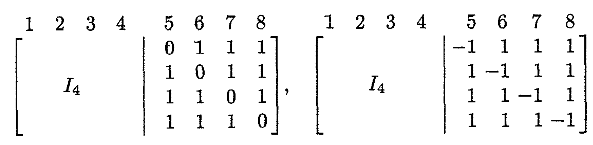
\includegraphics[width=12cm]{Test2/Problem7/FirstMatrices.png}
            \end{center}\pn
    
    \begin{enumerate}[label=(\roman*)]
        \item Show that $T_8$ and $R_8$ ar both self-dual.
        \item Show that $R_8$ is identically self-dual but $T_8$ is not.
        \item Give geometric representation for $T_8$ and $R_8$.
        \item Show that if $M \in \{T_8, R_8\}$ and $X = E(M) \setminus \{8\}$, then
                $(M|X)^* \cong F_7^-$.
        \item Consider the following matrices over $GF(3)$:
            \begin{center}
                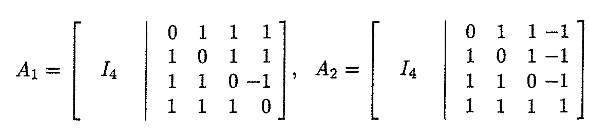
\includegraphics[width=12cm]{Test2/Problem7/SecondMatrices.png}
            \end{center}\pn
            Show, by applying a sequence of the row and clolumn opeartions to $A_1$ and $A_2$
            that $M[A_1] \cong T_8$ and $M[A_2] \cong R_8$.
        \item Show that $R_8$ can be obtained from $AG(3, 2)$ by relaxing two disjoint 
            circuit-hyperplanes.
    \end{enumerate}
}
\begin{proof}
\end{proof}
        \clearpage

    \section{Oxley, Section 2.3, Problem 1}
        \prob{}
\begin{proof}
\end{proof}
        \clearpage

    \section{Oxley, Section 2.3, Problem 2}
        \prob{}
\begin{proof}
\end{proof}
        \clearpage

    \section{Oxley, Section 2.3, Problem 6}
        \prob
{
    Construct the geometric duals of the plane graphs in the next figures.
		    \begin{center}
                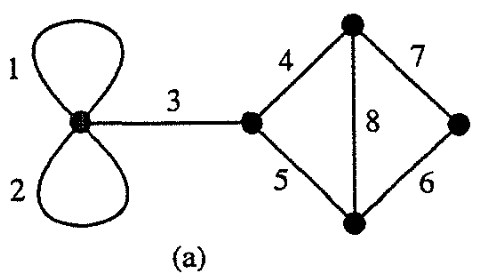
\includegraphics[width=5cm]{Test2/Problem10/Figure1_4.png}
            \end{center}\pn
						
			\begin{center}
                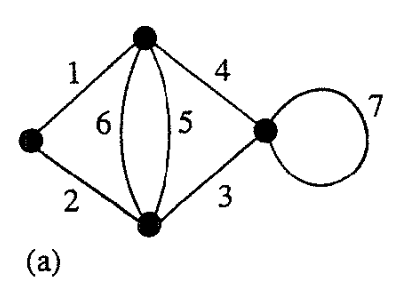
\includegraphics[width=5cm]{Test2/Problem10/Figure1_28.png}
            \end{center}\pn
}
\begin{proof}$\,$\pn
    \begin{figure}[H]
        \begin{center}
        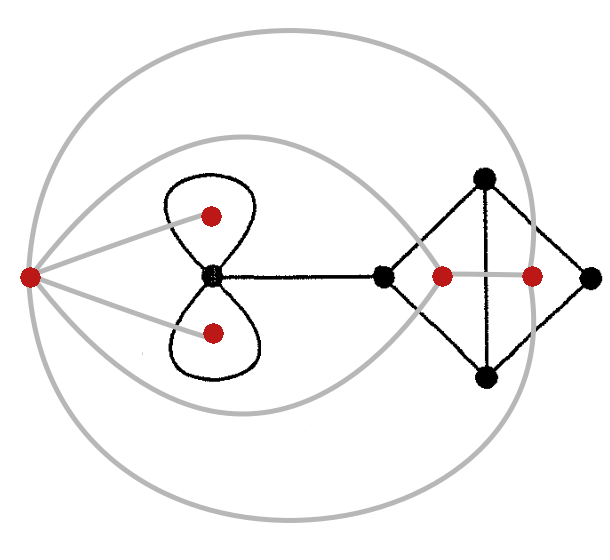
\includegraphics[width=5cm]{Test2/Problem10/Figure1_4_and_its_dual.png}
        \end{center}                            
        \caption{First graph and its dual}
        \label{t2:p9_Figure1_4_and_its_dual.png}                        
    \end{figure}\pn 
    
    \begin{figure}[H]
        \begin{center}
        \includegraphics[width=5cm]{Test2/Problem10/Figure1_4_dual.png}
        \end{center}                            
        \caption{First graph's dual}
        \label{t2:p9_Figure1_4_dual.png}                        
    \end{figure}\pn       
    
    \begin{figure}[H]
        \begin{center}
        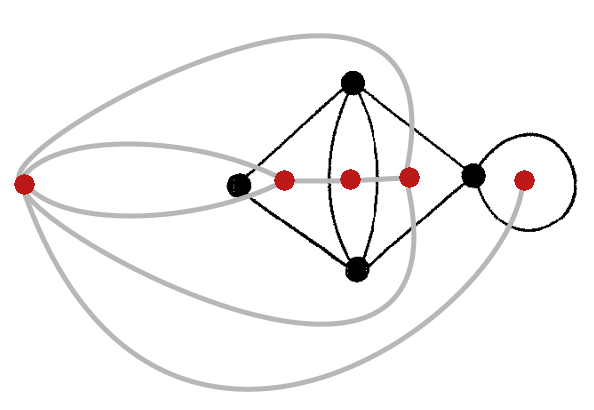
\includegraphics[width=5cm]{Test2/Problem10/Figure1_28_and_its_dual.png}
        \end{center}                            
        \caption{Second graph with its dual}
        \label{t2:p9_Figure1_28_and_its_dual.png}                        
    \end{figure}\pn   
        
    \begin{figure}[H]
        \begin{center}
        \includegraphics[width=5cm]{Test2/Problem10/Figure1_28_dual.png}
        \end{center}                            
        \caption{Second graph's dual}
        \label{t2:p9_Figure1_28_dual.png}                        
    \end{figure}\pn    
\end{proof}
        \clearpage

    \section{Oxley, Section 2.3, Problem 10}
        \prob{}
\begin{proof}
\end{proof}
        \clearpage

    \section{Oxley, Section 2.4, Problem 3}
        \prob
{
    Let $G$ be the directed graph shown in Figure 2.17(a).
            \begin{center}
                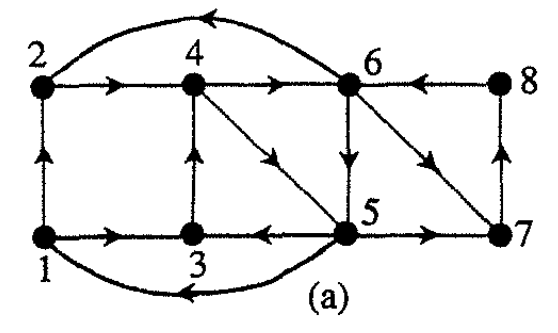
\includegraphics[width=5cm]{Test2/Problem12/DirectedGraphs.png}
            \end{center}\pn
    
    \begin{enumerate}[label=(\roman*)]
        \item   Construct the corresponding bipartite graph $\hat{G}$.
        \item   Let $V = \{1,2,3,4,5,6,7,8\}$, $X=\{5,7\}$, $Y=\{4,2\}$,
                and the paths linking $X$ to $Y$ in $G$ be 5134 and 7862. Construct the
                corresponding matching of $V \setminus X$ to $\hat{V} \setminus \hat{Y}$ in $\hat{G}$.
        \item   Now take the matching $\{2\hat{1}, 3\hat{5}, 4\hat{3}, 5\hat{4}, 6\hat{8}, 8\hat{7}\}$ in $\hat{G}$ and 
                construct the corresponding disjoint paths in $G$ as in the proof of Lemma 2.4.3.
    \end{enumerate}
}
\begin{proof}
\end{proof}
        \clearpage

    \section{Oxley, Section 2.4, Problem 4}
        \prob{}
\begin{proof}
\end{proof}
        \clearpage

    \section{Oxley, Section 3.1, Problem 1}
        \prob{}
\begin{proof}
\end{proof}
        \clearpage

    \section{Oxley, Section 3.1, Problem 4}
        \prob{}
\begin{proof}
\end{proof}
        \clearpage

    \section{Oxley, Section 3.2, Problem 3}
        \prob{}
\begin{proof}
\end{proof}
        \clearpage

    \section{Oxley, Section 3.2, Problem 5}
        \prob{}
\begin{proof}
\end{proof}
        \clearpage
